\label{Anforderungen}

Damit die Bewertung des Projektes erfolgreich wird, müssen zu Projektbeginn Anforderungen erarbeitet und festgelegt werden. Diese sind unveränderbar, da das Ergebnis sonst verfälschen würde. \\
Eine Anforderung muss zudem messbar und/oder überprüfbar sein, um deren Umsetzung später objektiv bewerten zu können. Somit wird auch eine sogenannte Verifikationsmethode festgelegt, mit der die Anforderungen später überprüft werden können. \\
Es wird zwischen sechs verschiedenen Verifikationsmethoden unterschieden:

\begin{itemize}
	\item Similarity: Suche und Abgleich mit bereits vorhandenen Lösungen \cite[S. 122]{HelgaMeyer.}
	\item Insparity: Soll- und Ist-Abgleich von Ein- und Ausgängen nach einem formalen Ablauf (Ein- und Ausgangskriterien sind vorher definiert) \cite[vgl. S. 308]{PeterLiggesmeyer.2009}
	\item Review: Soll- und Ist-Abgleich von Ein- und Ausgängen ohne formalen Ablauf (Ein- und Ausgangskriterien sind vorher nicht definiert) \cite[vgl. S. 317]{PeterLiggesmeyer.2009}
	\item Measurement: Durchführung einer Reihe von Operationen, die das Ziel haben, einen Wert einer quantitativen oder kategorialen Darstellung eines oder mehrerer Attribute zu bestimmen \cite[vgl. S. 395]{DepartmentofResearch&DevelopmentDepartmentofInformationTechnologiesandSystems.}
	\item Analysis: Basiert auf Heuristiken und Statistiken [...] [, die man] sich als starke Compiler-Typisierung [...] im Rahmen einer ausführlichen Datenfluss-Analyse vorstellen [kann] \cite[vgl. S. 4]{JayAbrahamPaulJonesRaoulJetley.}
	\item Test: Prüft und bewertet Software auf Erfüllung der für ihren Einsatz definierten Anforderungen und misst ihre Qualität \cite{Wikipedia.01.03.2020}
\end{itemize}

\newpage

Daher wurde am Anfang des Projektes eine Tabelle erstellt, indem alle Anforderungen definiert wurden. Zudem sind diese nummeriert und haben individuelle Verifikationsmethoden zugeordnet bekommen. \\

\begin{table}[!hbt]
	
	\centering
	
	\begin{tabular}{|r| p{8.4cm}|p{4.7cm}|}
		
		\hline
		Nummer & Anforderungen & Verifikationsmethode \\
		\hline
		1 & Echtzeitmessung der Luftgüte & Measurement \\
		\hline
		2 & Mindestmessbereich von 400 ppm bis 5000 ppm & Review \\
		\hline
		3 & Visualisierung der Luftgüte mithilfe von \ac{LED}s (gut, mittel, schlecht) & Test \\
		\hline
		4 & Ausgabe der Luftgüte mithilfe von \ac{LCD}-Display & Test \\
		\hline
		5 & Ansteuern eines Fensterscheibenmotors mithilfe einer \ac{LED} simulieren & Test \\
		\hline
		6 & Bei schlechter Luftgüte: Fenster öffnet sich (\ac{LED} an) & Test \\
		\hline
		7 & Bei guter Luftgüte: Fenster schließt sich (\ac{LED} aus) & Test \\
		\hline
		8 & Speichern im CSV-Format & Test, Analysis\\
		\hline
		9 & Zugriff auf Messdaten über SD-Karte & Test \\
		\hline
		10 & Benutzer kann zwischen drei Messprofilen auswählen (Messprofil: Abtastrate) & Test \\
		\hline
		
	\end{tabular}
	
	\captionabove{Anforderungen an das Projekt}
	\label{tab:Anforderungen}
	
\end{table}

Die Anforderungen sollen jedoch nicht nur mithilfe einer Tabelle und den dazugehörigen Verifikationsmethoden definiert werden. Wie in Abbildung \ref{fig:UseCase} zu sehen ist, wurde mithilfe von Architect Enterprise ein sogenanntes Use-Case-Diagramm erstellt, welches den Zusammenhang zwischen Anwender und Programmfunktionen aufzeigen soll. \\
Zu sehen ist, dass der Anwender zunächst zwischen zwei Funktionen wählen kann. So soll zum einen eine neue Messung gestartet werden können. Zum anderen soll der Benutzer in der Lage sein, dem Programm mitteilen zu können, dass die letzte Messung derzeit ausgelesen wird. \\
Im Fall, dass der Anwender eine neue Messung starten möchte, kann dieser, wie in Tabelle \ref{tab:Anforderungen} definiert wurde, zwischen drei Messprofilen wählen. \\
Falls der Benutzer dem Programm zu verstehen gegeben hat, die letzte Messung auslesen zu wollen, geht das Programm in einen Wartezustand. Hier wartet es so lange, bis der Anwender bestätigt hat, dass das Auslesen erfolgreich beendet wurde und die SD-Karte wieder ins Modul eingeführt wurde. \\

\begin{figure}[!hbt]
	\centering
	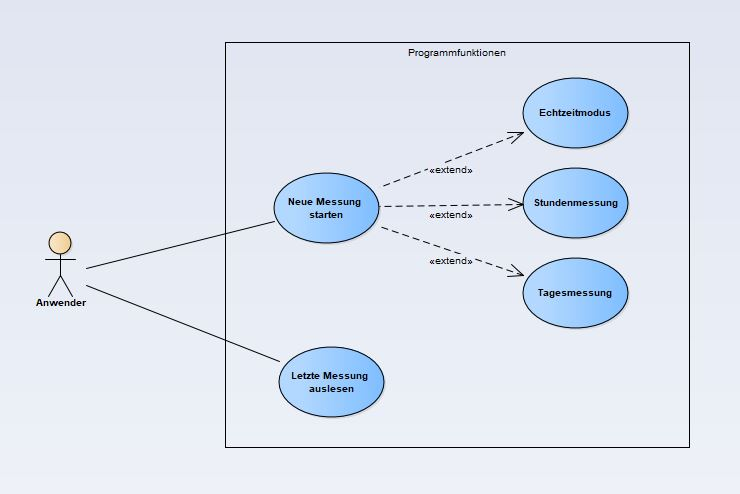
\includegraphics[width=0.9\linewidth]{Images/UseCase}
	\caption{Entwurf des Use-Case-Diagramms mithilfe von Enterprise Architect}
	\label{fig:UseCase}
\end{figure}